% !TEX Program = xelatex
\documentclass[print, doctor, vlined]{DissertUESTC}


\begin{document}
	
	\definecolor{shadcolor}{RGB}{228, 234, 246}
	\definecolor{notsored}{RGB}{139, 0, 0}
	\newcommand{\shad}[1]{\colorbox{shadcolor}{\ttfamily #1}}
	\newcommand{\shadcmd}[1]{\shad{\ttfamily $\backslash$#1}}
	
	\nocite{*}
	
	% 封面
%	\uestccover[<学院名称排版风格>]{<论文题目>}{<学科专业>}{<学号>}{<作者姓名>}{<指导教师>}{<教师职称>}{<学院>} % 学士、研究生通用
	\uestccover{关于我的杀父仇人疑似是名震天下的大侠时该如何报仇}
				{玉女素心剑法}
				{1182000}
				{杨\hspace{1em}过}
				{小龙女}
				{掌\hspace{1em}门}%{终南山古墓派}
				{终南山古墓派终南山古墓派终南山古墓派终南山古墓派}

	\uestccover[par]{关于我的杀父仇人疑似是名震天下的大侠时该如何报仇}
				{玉女素心剑法}
				{1182000}
				{杨\hspace{1em}过}
				{小龙女}
				{掌\hspace{1em}门}%{终南山古墓派}
				{终南山古墓派终南山古墓派终南山古墓派终南山古墓派}

	
	% 中文扉页,仅研究生用
	\ClsNum{TN828.6}  % \ClsNum{<分类号>}
	\ClsLv{公开}  % \ClsLv{<密级>}
	\UDC{621.39}  % \UDC{<UDC号>}
	\DissertationTitle{关于我的杀父仇人疑似是名震天下的大侠时该如何报仇}  % \DissertationTitle{<题名>}
	\Author{杨过}  % \Author{<作者姓名>}
	\Supervisor{小龙女}{掌门}{古墓派}{活死人墓}  % \Supervisor{<指导教师>}{<职称>}{<单位名称>}{<单位地址>}
	% 副导师信息,无则注释
	\AssociateSupervisor{洪七公}{前帮主}{丐帮}{襄阳}  % \AssociateSupervisor{<副导师名称>}{<职称}>{<单位名称>}{<单位地址>}
	\DegLv{西狂}  % \DegLv{<申请学位级别>},该信息由文档类选项自动确定,需修改默认内容时使用,否则注释即可
	\Major{玉女素心剑法}  % \Major{<学科专业>}
	\Profield{剑道}  % \Profield{专业学位领域代码},此为专业学位独有,学术学位用户注释即可
	\Date{1959年1月1日}{1961年1月1日}  % \Date{<论文提交日期>}{<论文答辩日期>}
	\Grant{中华武林}{1961年2月2日}  % \Grant{<学位授予单位>}{<学位授予日期>}
	\Reviewer{黄蓉}{一灯大师、老顽童、黄老邪、郭靖、小龙女}  % \Reviewer{<答辩委员为主席>}{<评阅人>}
	\uestczhtitlepage
	
	% 英文扉页,仅研究生用
	% \uestcentitlepage{<文题>}{<专业>}{<学号>}{<作者>}{<导师>}{<副导师>}{<学院>},若无副导师,则将“<副导师>”参数留空即可
	\uestcentitlepage{How to Take Revenge When My Father's Murderer is Suspected to Be a Famous Hero}
					{Jade Lady Soul Sword Technique}
					{1182000}
					{Yang Guo}
					{Grandmaster Dragondaughter Little}{Grandmaster Northern Beggar}
					{Ancient Tomb Sect}
	
	% 独创性声明:[签名宽度]{日期}{作者签名图片}{导师签名图片},送审时使用空强制参数即可,仅研究生用
	\declaration[3cm]{2024年08月31日}{authsign}{spvrsign}
	
	% 开启中文摘要
	\zhabstract
	
	杨过少年时期母亲染病而亡,随后他便过着四处流浪的生活。后来遇到郭靖夫妇,便由他们照看。但之后因杨过与郭芙等人之间的矛盾,郭靖便送其去全真派习武。其后,又从全真派逃出,机缘巧合下于古墓遇见小龙女,之后便跟随小龙女练功。 他身边有许多红颜知己钟情于他,而他却一心只爱小龙女,后结为夫妇;他和郭家恩怨难分,数度因误会关系紧张,却始终挺身而出相助他们,解除嫌隙,化气为和;命运多舛,与小龙女分隔十六年里,随伴亦师亦友的神雕行侠仗义,惩恶扬善。江湖人称“神雕大侠”。 后等小龙女不至毅然跳崖殉情,在谷底与小龙女重逢后携手保卫襄阳城,杨过一展其旷世武学的威力,打败金轮法王,飞石击杀蒙古大汗,保大宋十三年和平。成为名扬天下的“神雕侠侣”。 最后一次华山论剑后,与妻子小龙女绝迹江湖。
	
	% 中文关键字
	\zhkeywords{练武,离经叛道,复仇,抗敌,练武,离经叛道,复仇,抗敌,练武,离经叛道,复仇,抗敌,练武,离经叛道,复仇,抗敌}
	
	
	% 开启英文摘要
	\enabstract
	
	When Yang was a teenager, his mother contracted a disease and died, and he then lived a wandering life. When he met Guo Jing and his wife, they took care of him. However, due to the conflict between Yang and Guo Fu, Guo Jing sent him to learn martial arts in the Quanzhen Sect. Later, he escaped from the Quanzhen Sect and met Xiao Longnian at the ancient tomb, where he practised kung fu with Xiao Longnian. He was surrounded by many confidantes who were in love with him, but he only loved Little Dragon Girl, and later married; he and the Guo family feud, several times due to misunderstanding tension, but always stepped forward to help them, lifting the suspicion, turning the gas into peace; ill-fated, separated from Little Dragon Girl for sixteen years, along with the Divine Eagle who is also a teacher and friend of the chivalrous, punishing the evil and promoting the good. Jianghu people ``divine eagle hero". After the little dragon lady is not to perseverance to jump off the cliff to martyrdom, in the bottom of the valley and the little dragon lady reunited with the defence of Xiangyang City, Yang past a show of its unparalleled martial arts power to defeat the Golden Wheel of the Fa Wang, flying stone to kill the Mongolian Khan, to protect the thirteen years of peace in the Great Song Dynasty. He became the world-famous ``Divine Eagle Couple". After the last Mount Hua sword debate, he and his wife Xiaolongnu went into exile.
	
	
	% 英文关键字
	\enkeywords{Martial arts, apostasy, revenge, fighting against the enemy, martial arts, apostasy, revenge, fighting against the enemy}
	
	\tableofcontents  % 主目录,必要
	
	\listoffigures  % 图多则放,反之不放
	
	\listoftables  % 表多则放,反之不放
	
	\listofsymbs  % 生成主要符号表标题,需要额外维护符号表内容
	
	生成主要符号表的章标题需使用本模板提供的\shadcmd{listofsymbs}命令。排版主要符号表的内容则需要使用本模板提供的\shad{symbtable}环境。该环境基于\shad{longtable}环境进行封装,依次接受两个可选参数:
	
	\shadcmd{begin\{symbtable\}[<表格整体位置>](<主要符号表的列控制参数>)}
	
	\noindent 其中,第一项可选参数用于设置\shad{longtable}环境的可选参数,且默认值与\shad{longtable}环境保持一致;第二项可选参数用于设置\shad{longtable}环境的必选参数,其默认值设置为\shad{p\{3.5em\} p\{$\backslash$linewidth-9em\} p\{3em\}<\{$\backslash$centering\}}。
	
	若非必要,用户不应指定\shad{symbtable}环境的可选参数。但若出于对排版美观性的考虑,可适当调整主要符号表各列的宽度。注意,按照学位论文撰写规范中的示例,\textbf{主要符号表有且仅有三列}。因此,切勿对第二项可选参数设置其他列数。
	
	\textbf{重要提醒}:\shadcmd{listofsymbs}命令和\shad{symbtable}环境必须同时出现或消失。消失好理解,不需要主要符号表的时候,通通注释掉即可;需要的时候,必须使用\shad{symbtable}环境生成表格内容,因为在印刷模式下,这部分结束时是否需要添加左手空白页的判断逻辑放在了\shad{symbtable}环境结束时(自动)执行。
	
	\begin{symbtable}
		a & 加速度(acceleration) & 1 \\
		A & 振幅(amplitude)、面积(Area)、磁场矢量势(magnetic vector potential) & 2 \\
		B & 磁场、磁感应强度、核结合能 & 3 \\
		c & 真空中光速 & 4 \\
		C & 比热容(heat capacity)、电容 & 5 \\
		d & 长度(distance)、直径(diameter)、微分(differential,如dx)& 6 \\
		D & 电位移矢量(electric displacement) & 7 \\
		e & 元电荷、自然底数(欧拉常数)& 8 \\
		E & 能量、电场场强,电动势 & 9 \\
		f & 频率、焦距(光学) & 10 \\
		F & 力、通量(Flux) & 11 \\
		g &(地表)重力加速度 & 12 \\
		G & 万有引力常数 & 13 \\
		h & 普朗克常数、高度 & 14 \\
		H & 哈勃常数、焓、磁化强度矢量、哈密顿算符(Hamiltonian) & 15 \\
		i & 虚数单位 & 16 \\
		I & 电流、惯量(inertia)、冲量(impulse) & 17 \\
		j & 辐射强度、加加速度(jerk) & 18 \\
		J & 角动量、概率流(量子力学)、电流密度、巨配分函数里的巨势 Z(J) & 19 \\
		k & 玻尔兹曼(Boltzmann)常数、库伦常数、用来指代某常量或固定比值 & 20 \\
		K & 四维波矢量(相对论)、动能 & 21 \\
		l & 长度(length) & 22 \\
		L & 角动量、电感系数 & 23 \\
		m & 质量 & 24 \\
		M & 磁化率 & 25 \\
		n & 序数、主量子数、摩尔数(化学)、折射率(光学) & 26 \\
		N & 序数、中子数、放大倍率(光学)& 27 \\
		o & 小o符号 & 28 \\
		O & 大O符号 & 29 \\
		p & 动量、压强(pressure)、电偶极矩(electric dipole moment) & 30 \\
		P & 概率(量子力学,统计学)、功率(power)、极化度 & 31 \\
		q & 电荷 & 32 \\
		Q & 电荷热量、流量 & 33 \\
		r & 半径、位置向量、球坐标系半径轴 & 34 \\
		R & 电阻、普适气体常数(热力学)、里德伯(Rydberg)常数(光谱学)、反射率(Reflectivity,光学) & 35 \\
		s & 自旋 & 36 \\
		S & 熵、面积 & 37 \\
		t & 时间 & 38 \\
		T & 温度、周期、透射率(Transmittance,光学) & 39 \\
		u & 原子质量单位、物距(光学) & 40 \\
		U & 电压、电势 & 50 \\
		v & 速度、像距(光学) & 51 \\
		V & 体积、势能 & 52 \\
		w & 速度 & 53 \\
		W & 功 & 54 \\
		x & 直角坐标系横轴 & 55 \\
		X & 磁化率、电抗 & 56 \\
		y & 直角坐标系纵轴 & 57 \\
		Y & 光亮度、球谐函数 & 58 \\
		z & 直角/圆柱坐标系竖轴、复数变量 & 59 \\
		Z & 阻抗、原子序数(质子数)、配分函数(partition function) & 60 \\
		$\alpha$ & 角度、精细结构常数、角加速度、四维加速度(相对论)、攻角 & 61 \\
		Α & Alpha (与英文拼写难区分的希腊字母一般不使用) & 62 \\
		$\beta$ & 角度;磁通系数;速度与光速的比值 & 63 \\
		Β & Beta Β函数 & 64 \\
		γ & 电导系数、洛伦兹因子、热容比 & 65 \\
		Γ & Gamma Γ函数、克里斯托弗尔符号 & 66 \\
		δ & 狄拉克δ函数、克罗内克函数(Kronecker delta)、屈光度、微分 & 67 \\
		Δ & Delta 拉普拉斯算子、有限差 & 68 \\
		ε & 电容率(permittivity)、介电常数、列维-奇维塔符号(Levi-Civita symbol)、发射率 & 69 \\
		Ε & Epsilon & 70 \\
		Ϝ & digamma & 71 \\
		ζ & 阻尼比、黎曼ζ函数 & 72 \\
		Ζ & Zeta & 73 \\
		η & 黏度(viscosity)、磁滞系数、效率 & 74 \\
		Η & Eta & 75 \\
		θ & 角变量、温度、球坐标/圆柱坐标横角 & 76 \\
		Θ & Theta 单位阶跃函数(Heaviside step function) & 77 \\
		Ι & Iota & 78 \\
		$\kappa$ & 介质常数比ε/ε0、导热率、热扩散率 & 79 \\
		$\kappa$ & Kappa & 80 \\
		λ & 波长、mean free path、半衰期 & 81 \\
		$\Lambda$ & Lambda 洛伦兹变换、冯·卡门常数 & 82 \\
		μ & 磁导率、质子质量单位、摩擦系数、离子迁移率 & 83 \\
		Μ & Mu & 84 \\
		ν & 频率、运动粘度、自由度 & 85 \\
		Ν & Nu & 86 \\
		ξ & 黎曼ξ函数、随机变量 & 87 \\
		Ξ & Xi & 88 \\
		Ο & Omicron & 89 \\
		π & 圆周率、共轭动量 & 90 \\
		∏ & Pi 乘积 & 91 \\
		ρ & 密度、电阻率 & 92 \\
		Ρ & Rho & 93 \\
		σ & 导电率、斯提芬-波尔兹曼常数(Stefan–Boltzmann constant)、核反应截面、表面密度、标准差 & 94 \\
		∑ & Sigma 总和 & 95 \\
		τ & 扭矩(Torque)、剪应力(Shear stress)、时间常数、2π & 96 \\
		Τ & Tau & 97 \\
		Υ & Upsilon & 98 \\
		φ & 球坐标纵角、波相位(wave phase)、直径 & 99 \\
		Φ & Phi 磁通量、辐射通量、逸出功 & 100 \\
		χ & 电极化率(Electric susceptibility) & 101 \\
		Χ & Chi 电抗 & 102 \\
		ψ & 角速;介质电通量(静电力线) & 103 \\
		Ψ & Psi 波函数 & 104 \\
		ω & 角速度 & 105 \\
		Ω & omega 蔡廷常数(Chaitin's constant) 立体角(Solid angle) & 106 \\
	\end{symbtable}
	
	
	
	% 打印缩略词表,\printnomenclature[<英文缩写宽度>](<中文全称宽度>)
	\printnomenclature
	\nomchn{LP}{Linear Programming}{线性规划}  % 创建缩略词条目,% \nomchn{<缩略词>}{<英文全称>}{<中文全称>}
	\nomchn{PLE}{Path Loss Exponent}{路径损失指数}
	\nomchn{QoS}{Quality of Service}{服务质量}
	\nomchn{SLA}{Service Level Agreement}{服务水平协议}
	\nomchn{NLP}{non-linear programming}{非线性规划}
	
	生成缩略词表相对复杂一些:
	\begin{enumerate}
		\item 先使用\shadcmd{printnomenclature[<英文缩写宽度>](<中文全称宽度>)},第一项可选参数控制\textbf{英文缩写}的列宽,默认为\shad{5em};第二项可选参数控制\textbf{中文全称}的列宽,默认为\shad{7.5em}。
		
		\item 然后在正文中出现缩略词的位置使用命令\\\shadcmd{nomchn\{<缩略词>\}\{<英文全称>\}\{<中文全称>\}}添加该缩略词条目。
	\end{enumerate}
	
	另外,本地用户需要先编译生成缩略词表的辅助文件,再编译完整文档才能获得正确的结果,教程参见\href{https://zhuanlan.zhihu.com/p/46442713}{\shad{编译缩略词表}}。Overleaf用户则可以一键搞定,无需额外操作。
	
	细心的朋友可能会发现,在印刷模式下,当前段落所在的页并未标注任何页眉与页脚,猜猜为什么。不必慌张,在你正式使用本模板撰写论文时,肯定不需要当前页的内容。
	
	\chapter{模板使用说明}
	
	\section{导言区及模板选项}

	模板的导言区只有两行:
	\begin{itemize}
		\item \shad{\% !TEX Program = xelatex}在Texstudio中表示指定使用XeLaTeX编译该文档,对其他编辑器,可能需要用户手动设置编译引擎。

		\item \shadcmd{documentclass[<选项列表>]\{DissertUESTC\}}表示加载名为\shad{DissertUESTC}的文档类,该文档类基于LaTeX的\shad{book}类编写。此文档类新增四种选项:

		\begin{itemize}
			\item \shad{print}/\shad{nonprint}:该选项控制是否以印刷模式生成文档,印刷模式会自动在论文的前置部分添加必要的空白页。默认为\shad{print}。

			\item \shad{doctor}/\shad{prodoctor}/\shad{master}/\shad{promaster}/\shad{bachelor}:该选项设置学位论文类型,分别对应学术学位博士、专业学位博士、学术学位硕士、专业学位硕士以及学士学位。默认为`doctor`。
   
			\item \shad{subfigsimple}/\shad{subfigparens}:该选项用于调整正文中对子图标签进行引用生成的编号样式,\shad{subfigsimple}对应样式为\shad{1-1a},\shad{subfigparens}对应样式为\shad{1-1(a)},默认为\shad{subfigparens}。
   
			\item \shad{draftfig}:LaTeX标准文档类提供的\shad{draft}选项在排版草稿时不会生成交叉引用链接、超链接、书签,图片也会被替换为尺寸与之相同的方框+文本,并且会在超出表格、页面边界的位置标注粗框线。\shad{draftfig}选项则仅将图片替换为方框+文本,而不修改标准\shad{draft}选项涉及的其他内容。其主要用处是在自行查重时便捷地隐去论文中的图片,而不影响排版。

			\item 另外,\shad{algorithm2e}宏包的\shad{vlined}和\shad{boxruled}选项也可以在加载文档类时设置。
		\end{itemize}
	\end{itemize}
	
	\section{各级标题}
	
	本模板基于\shad{book}类,章标题需要使用\shad{$\backslash$chapter\{<章标题>\}} 生成,其他各级标题依次为\shad{$\backslash$section\{<节标题>\}}、\shad{$\backslash$subsection\{<子节标题>\}}、\\ \shad{$\backslash$subsubsection\{<孙节标题>\}}。
	
	\section{图片}
	
	本模板使用graphicx和subfig宏包来处理插入的图片及子图,需要将待排版图片文件放入项目目录\shad{./fig/}中。以下给出一些排版图片的例子。
	
	\begin{figure}[!htb]
		\centering
		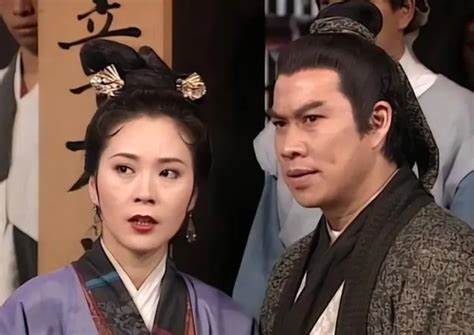
\includegraphics[width=0.7\linewidth]{黄蓉郭靖1}
		\caption{锁定仇人}
	\end{figure}
	
	\clearpage
	\begin{figure}[!htb]
		\centering
		\subfloat[]{
			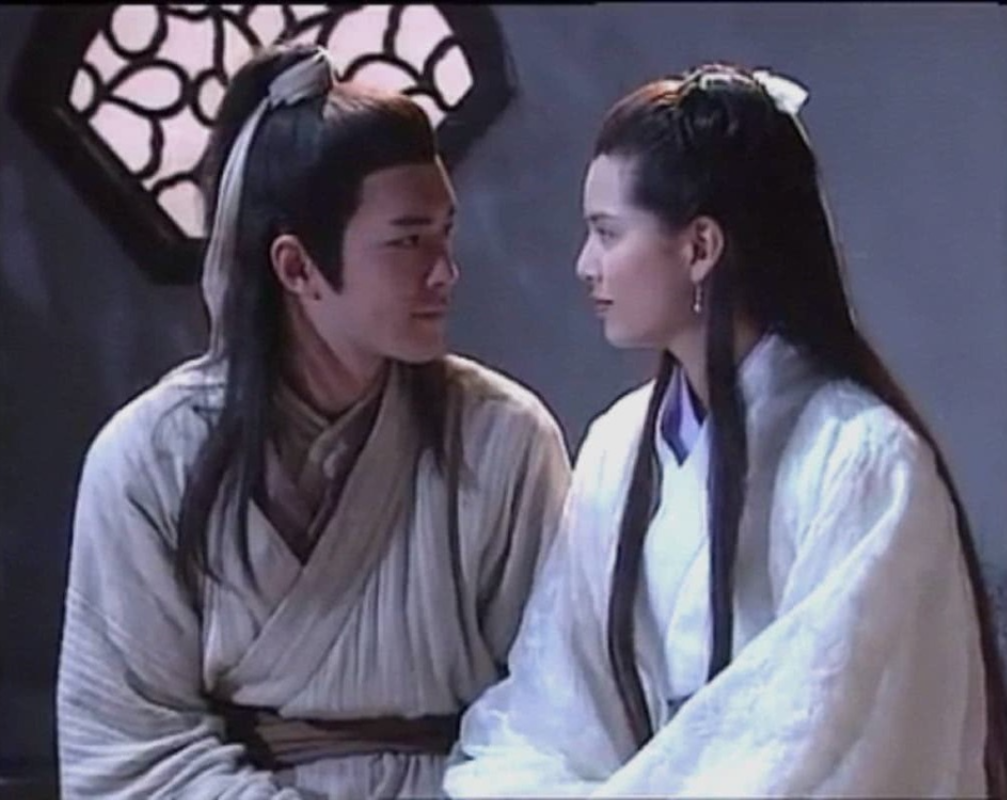
\includegraphics[width=0.4\linewidth]{杨过小龙女3}
			\label{fig: 见到姑姑嘻嘻}
		}
		\hfill
		\subfloat[]{
			
\includegraphics[width=0.4\linewidth]{杨过小龙女6}
			\label{fig: 姑姑见我不嘻嘻}
		}
		\caption[报仇哪有姑姑重要]{报仇哪有姑姑重要。\subref{fig: 见到姑姑嘻嘻}见到姑姑我嘻嘻;\subref{fig: 姑姑见我不嘻嘻}姑姑见我不嘻嘻} \label{fig: 报仇哪有姑姑重要}
	\end{figure}
	

	需要注意,图\ref{fig: 报仇哪有姑姑重要}中引用子图\ref{fig: 见到姑姑嘻嘻}和本段中引用子图使用的命令分别为\shad{$\backslash$subref\{fig: 见到姑姑嘻嘻\}}和\shad{$\backslash$ref\{fig: 报仇哪有姑姑重要\}},它们分别生成仅含带括号子图编号和完整子图编号的结果。
	
	另外,图\ref{fig: 报仇哪有姑姑重要}的图题包含了子图题文本,但生成的图目录中却只有主图题文本,其实现方式为在主图题命令中使用可选参数单独指定图目录中的显示文本:\shad{$\backslash$caption[报仇哪有姑姑重要]}
	
	\begin{figure}[!htb]
		\centering
		\subfloat[]{
			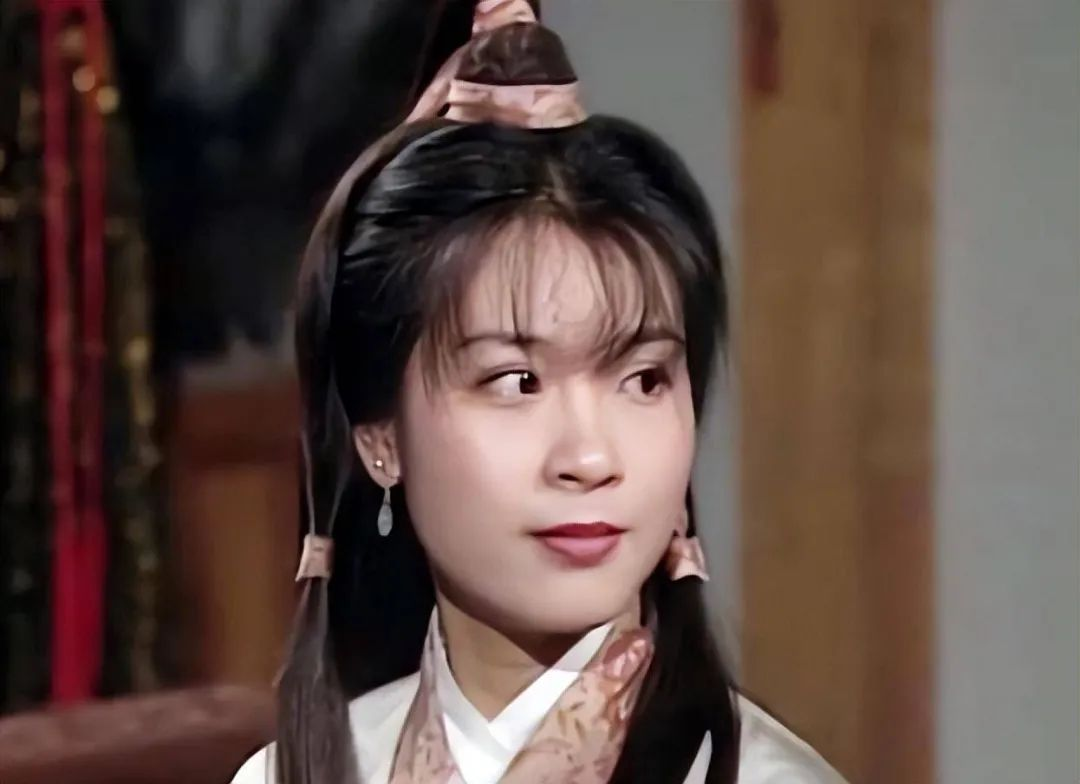
\includegraphics[width=0.4\linewidth]{陆无双2}
			\label{fig: 陆无双2}
		}
		\hfill
		\subfloat[]{
			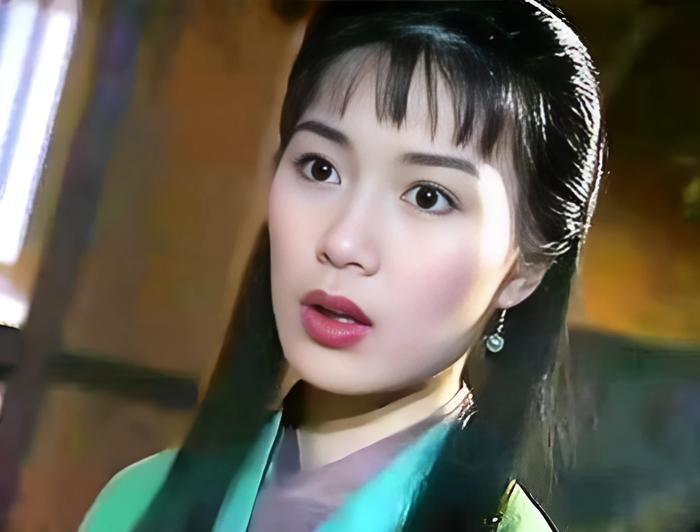
\includegraphics[width=0.4\linewidth]{程英3}
			\label{fig: 程英3}
		}
		\caption{找其他红颜知己嘻嘻。\subref{fig: 陆无双2}眼睛像姑姑;\subref{fig: 程英3}举止像姑姑} \label{fig: 红颜知己}
	\end{figure}
	
	\begin{figure}[!htb]
		\centering
		\subfloat[]{
			
\includegraphics[width=0.4\linewidth]{绿萼2}
			\label{fig: 绿萼2}
		}
		\hfill
		\subfloat[]{
			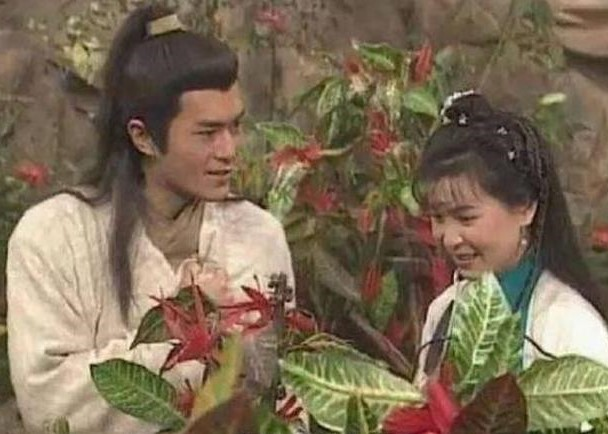
\includegraphics[width=0.4\linewidth]{杨过绿萼}
			\label{fig: 杨过绿萼}
		}
		\\
		\subfloat[]{
			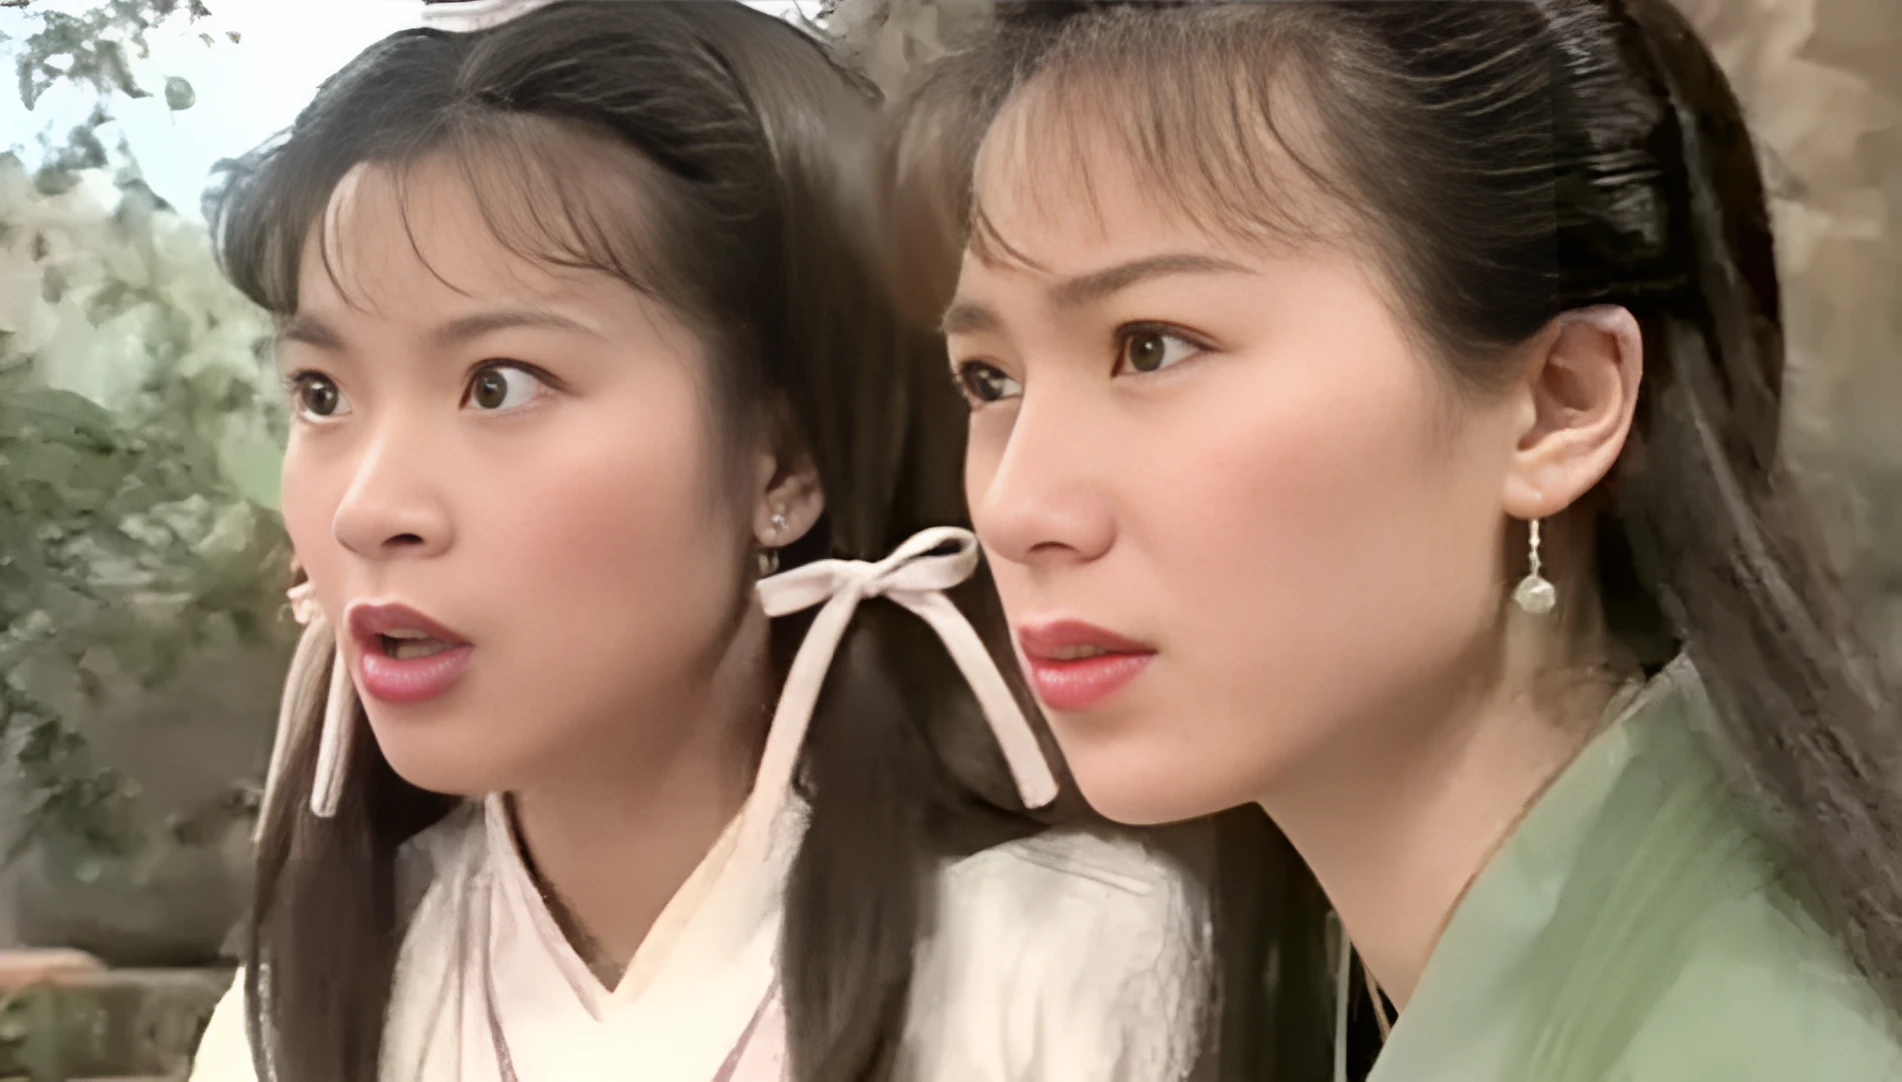
\includegraphics[width=0.98\linewidth]{陆无双程英}
			\label{fig: GG}
		}
		\caption{撩妹是我杨过的被动技能。\subref{fig: 绿萼2}好腼腆的姑娘;\subref{fig: 杨过绿萼}你终于肯笑了;\subref{fig: GG}哦吼} \label{fig: 被动技能}
	\end{figure}

	研究生和本科生学位论文规范对多行图题左右侧缩进距离的要求不同,前者为单侧\shad{4em},后者为单侧\shad{2em}。此参数由论文类型选项控制,无需用户过问。各位可以试试看,图\ref{fig: 被动技能}的主图题在\shad{bachelor}选项下能单行排版,而在其他类型选项下会换行。
	
	\begin{figure}[!htb]
		\centering
		
\includegraphics[width=0.9\linewidth]{杨过郭靖}
		\caption{还是推主线吧,动手动手}
	\end{figure}
	
	\clearpage
	\section{表格}
	
	\subsection{普通表格}
	
	普通表格的排版本身无需多言,使用\shad{table}+\shad{tabular}环境即可,但是要注意三线表中的三条线分别需要使用\shad{$\backslash$toprule}、\shad{$\backslash$midrule}、\shad{$\backslash$bottomrule}生成,这样才符合研究生规范中对线高的要求(\shad{1.5}磅、\shad{0.75}磅、\shad{1.5}磅)。注意不要用\shad{$\backslash$hline}。而对于本科生,学士学位论文规范要求表格中的线高统一为\shad{0.5}磅,在\shad{bachelor}选项下,\shad{$\backslash$midrule}的线高设置为\shad{0.5}磅。因此,本科生在表格中只需要也只可以使用\shad{$\backslash$midrule}和\shadcmd{cmidrule},否则线高将不符合要求。
	
	在需要为表格中的某些单元格添加水平框线时,应使用\newline\shadcmd{cmidrule[<线高>](<修剪>)\{<起始列-终止列>\}}而非\shadcmd{cline\{<起始列-终止列>\}}。后者似乎无法调整线高,也无法对框线的端点进行修剪。前者的第一项可选参数允许用户设置框线高度,其默认值在\shad{bachelor}选项下设置为了\shad{0.5}磅,而在其他论文类型下设置为了\shad{0.75}磅。如非必要,用户无需设置该可选参数;第二项可选参数允许用户对框线的端点进行修剪,当需要避免同行独立的相邻框线在视觉上连通到一起时,该选项将很有用,比如表\ref{tab: cmidrule示例}中的示例。有关第二项可选参数可取的值,建议用户查阅\shad{booktabs}宏包的官方文档。
	
	\begin{table}[htbp]
		\caption{$\backslash$cmidrule示例}\label{tab: cmidrule示例}
		\begin{threeparttable}
			\begin{tabular}{ccccc}
				\toprule
				\multirow{2}{*}{Column0} &  \multicolumn{2}{c}{Column1\tnote{1}} & \multicolumn{2}{c}{Column2\tnote{2}} \\
				\cmidrule(lr){2-3}\cmidrule[2.5bp](l){4-5}
				~     & subcolumn1 & subcolumn2 & subcolumn1 & subcolumn2 \\
				\midrule
				Row1  & element11 & element12 &element13 & element14 \\
				Row2  & element21 & element22 &element23 & element24 \\
				\cmidrule{2-3}\cmidrule[2.5bp]{4-5}
				Row3  & element31 & element32 &element33 & element34 \\
				\bottomrule
			\end{tabular}
			\begin{tablenotes}
				\item[1] 在\shad{bachelor}选项下,\shadcmd{cmidrule}默认线高设置为0.5bp,而在其他论文类型下,默认值为0.75bp,两者规范的要求不同。可用第二项可选参数同时修剪掉框线的左右端点
				\item[2] 通过指定\shadcmd{cmidrule}的第一项可选参数调整线高,并用第二项可选参数仅修剪掉框线的左端点
			\end{tablenotes}
		\end{threeparttable}
	\end{table}
	
	\newpage
	\subsection{带附注表格}
	
	更需要说明的是生成带附注的表格。本模板采用\shad{threeparttable}宏包实现将表格中的附注内容顶格排版在表格底部:
	\begin{enumerate}
		\item 使用\shadcmd{tnote\{<label>\}}在表格中插入上标编号;
		\setcounter{enumi}{98}
		\item 使用\shad{tablenotes}环境在表格底部排版附注。该环境提供选项\shad{online}用于将附注文本前的标号从默认的上标样式(见表\ref{tab: 江湖势力背调})更改为非上标样式(见表\ref{tab: 已习得武功})。
	\end{enumerate}
	
	\begin{table}[!ht]
		\caption{江湖势力背调} \label{tab: 江湖势力背调}
		\begin{threeparttable}
			\begin{tabular}{p{2cm} p{3cm} p{7cm}}
				\toprule
				\textbf{姓名} & \textbf{所属势力} & \textbf{武功绝学} \\
				\midrule
				郭靖 & 重阳宫 & 降龙十八掌 \\
				黄蓉 & 丐帮 & 打狗棒法 \\
				洪七公 & 丐帮 & 降龙十八掌、打狗棒法 \\
				黄老邪 & 桃花岛 & 弹指神通、落英神剑掌、玉箫剑法 \\
				老顽童 & 重阳宫 & 左右互博术\tnote{1} \\
				一灯 & 云南大理 & 一阳指\tnote{2}、千里传音 \\
				\bottomrule
			\end{tabular}
			\begin{tablenotes}
				\item[1] 自创武功
				\item[2] 云南大理段氏嫡传的武功,在点穴功夫中位居天下第一,运功后以右手食指点穴,出指可缓可快,缓时潇洒飘逸,快则疾如闪电,但着指之处,分毫不差。当与敌挣搏凶险之际,用此指法既可贴近径点敌人穴道,也可从远处欺近身去,一中即离,一攻而退,实为克敌保身的无上妙术。
			\end{tablenotes}
		\end{threeparttable}
	\end{table}
	
	\begin{table}[!ht]
		\caption{已习得武功} \label{tab: 已习得武功}
		\begin{threeparttable}
			\begin{tabular}{p{3cm} p{3cm} p{5cm}}
				\toprule
				\textbf{武功绝学} & \textbf{传授者} & \textbf{传授地点} \\
				\midrule
				蛤蟆功 & 欧阳锋 & 重阳山脉 \\
				九阴真经 & 小龙女 & 活死人墓 \\
				打狗棒法 & 洪七公、黄蓉 & 华山之巅、英雄大会 \\
				玉箫剑法 & 黄老邪 & 深山老林 \\
				黯然销魂掌\tnote{1} & 自创 & 海边 \\
				\bottomrule
			\end{tabular}
			\begin{tablenotes}[online]
				\item[1] 黯然销魂掌,是在杨过与小龙女离别后,认为今生再也见不到小龙女,悲从中来,由此创作了黯然销魂掌。黯然销魂掌和心情有关,此后杨过与小龙女重逢后,其心理愉悦,故使不出黯然销魂掌。
			\end{tablenotes}
		\end{threeparttable}
	\end{table}
	
	
	\clearpage
	\subsection{跨页表格}
	
	原则上,长度不足一页的表格不应跨页。而对于本身超过一页的表格,本模板使用\shad{longtable}宏包提供的\shad{longtable}环境实现。用户需要了解\shad{longtable}环境的基本使用方法,它与\shad{tabular}环境的最大区别在于需要用户自行定义分页后的表题、表头以及表尾。本模板提供了命令\shadcmd{CPcaption\{<跨页表题>\}}来正确排版跨页之后的表题,务必使用此命令,否则跨页后的表题将会与表格内容采用相同的行距和段前段后,而非与规范中要求的表题格式保持一致。
	
	此外,不应将\shad{longtable}环境嵌套在\shad{table}等浮动环境中,否则长表格将无法正常跨页。具体细节参见下方示例表\ref{tab: 中国计算机学会部分推荐期刊及会议}。
	
	\begin{longtable}{p{2em} p{4.5em} p{11em} p{6em} p{11em}}
		\caption{中国计算机学会部分推荐期刊及会议} \label{tab: 中国计算机学会部分推荐期刊及会议} \\
		
		\toprule
		\textbf{序号} & \textbf{刊物简称} & \textbf{刊物全称} & \textbf{出版社} & \textbf{网址} \\
		\midrule
		\endfirsthead
		
		% 在这里设计首页以外的表题和表头
		\multicolumn{5}{c}{\CPcaption{中国计算机学会部分推荐期刊及会议}}\\
		\toprule
		\textbf{序号} & \textbf{刊物简称} & \textbf{刊物全称} & \textbf{出版社} & \textbf{网址} \\
		\midrule
		\endhead
		
		% 在这里设计首页以外的表尾
		\bottomrule
		& & & & \hfill 续下页 \\  % 如不希望跨页表尾显示任何内容则注释掉即可
		\endfoot
		
		\bottomrule
		\endlastfoot
		
		1 & JSAC & IEEE Journal on Selected Areas in Communications & IEEE & http://dblp.uni-trier.de/db/journals/jsac/ \\
		2 & TMC & IEEE Transactions on Mobile Computing & IEEE & http://dblp.uni-trier.de/db/journals/tmc/ \\
		3 & TON & IEEE/ACM Transactions on Networking & IEEE/ACM & http://dblp.uni-trier.de/db/journals/ton/ \\
		1 & TOIT & ACM Transactions on Internet Technology & ACM & http://dblp.uni-trier.de/db/journals/toit/ \\
		2 & TOMM & ACM Transactions on Multimedia Computing, Communications and Applications & ACM & http://dblp.uni-trier.de/db/journals/tomccap/ \\
		3 & TOSN & ACM Transactions on Sensor Networks & ACM & http://dblp.uni-trier.de/db/journals/tosn/ \\
		4 & CN & Computer Networks & Elsevier & http://dblp.uni-trier.de/db/journals/cn/ \\
		5 & TCOM & IEEE Transactions on Communications & IEEE & http://dblp.uni-trier.de/db/journals/tcom/ \\
		6 & TWC & IEEE Transactions on Wireless Communications & IEEE & http://dblp.uni-trier.de/db/journals/twc/ \\
		1 & & Ad Hoc Networks & Elsevier & http://dblp.uni-trier.de/db/journals/adhoc/ \\
		2 & CC & Computer Communications & Elsevier & http://dblp.uni-trier.de/db/journals/comcom/ \\
		3 & TNSM & IEEE Transactions on Network and Service Management & IEEE & http://dblp.uni-trier.de/db/journals/tnsm/ \\
		4 & & IET Communications & IET & http://dblp.uni-trier.de/db/journals/iet-com/ \\
		5 & JNCA & Journal of Network and Computer Applications & Elsevier & http://dblp.uni-trier.de/db/journals/jnca/ \\
		6 & MONET & Mobile Networks and Applications & Springer & http://dblp.uni-trier.de/db/journals/monet/ \\
		7 & & Networks & Wiley & http://dblp.uni-trier.de/db/journals/networks/ \\
		8 & PPNA & Peer-to-Peer Networking and Applications & Springer & http://dblp.uni-trier.de/db/journals/ppna/ \\
		9 & WCMC & Wireless Communications and Mobile Computing & Wiley & http://dblp.uni-trier.de/db/journals/wicomm/ \\
		10 & & Wireless Networks & Springer & http://dblp.uni-trier.de/db/journals/winet/ \\
		11 & IOT & IEEE Internet of Things Journal & IEEE & https://dblp.org/db/journals/ iotj/index.html \\
		1 & SIGCOMM & ACM International Conference on Applications, Technologies, Architectures, and Protocols for Computer Communication & ACM & http://dblp.uni-trier.de/db/conf/sigcomm/ index.html \\
		2 & MobiCom & ACM International Conference on Mobile Computing and Networking & ACM & http://dblp.uni-trier.de/db/conf/mobicom/ \\
		3 & INFOCOM & IEEE International Conference on Computer Communications & IEEE & http://dblp.uni-trier.de/db/conf/infocom/ \\
		4 & NSDI & Symposium on Network System Design and Implementation & USENIX & http://dblp.uni-trier.de/db/conf/nsdi/ \\
		1 & SenSys & ACM Conference on Embedded Networked Sensor Systems & ACM & http://dblp.uni-trier.de/db/conf/sensys/ \\
		2 & CoNEXT & ACM International Conference on Emerging Networking Experiments and Technologies & ACM & http://dblp.uni-trier.de/db/conf/conext/ \\
		3 & SECON & IEEE International Conference on Sensing, Communication, and Networking & IEEE & http://dblp.uni-trier.de/db/conf/secon/ \\
		4 & IPSN & International Conference on Information Processing in Sensor Networks & IEEE/ACM & http://dblp.uni-trier.de/db/conf/ipsn/ \\
		5 & MobiSys & ACM International Conference on Mobile Systems, Applications, and Services & ACM & http://dblp.uni-trier.de/db/conf/mobisys/ \\
		6 & ICNP & IEEE International Conference on Network Protocols & IEEE & http://dblp.uni-trier.de/db/conf/icnp/ \\
		7 & MobiHoc & International Symposium on Theory, Algorithmic Foundations, and Protocol Design for Mobile Networks and Mobile Computing & ACM/IEEE & http://dblp.uni-trier.de/db/conf/mobihoc/ \\
		8 & NOSSDAV & International Workshop on Network and Operating System Support for Digital Audio and Video & ACM & http://dblp.uni-trier.de/db/conf/nossdav/ \\
		9 & IWQoS & IEEE/ACM International Workshop on Quality of Service & IEEE & http://dblp.uni-trier.de/db/conf/iwqos/ \\
		10 & IMC & ACM Internet Measurement Conference & ACM/USENIX & http://dblp.uni-trier.de/db/conf/imc/ \\
		
	\end{longtable}
	
	\clearpage
	\section{伪代码}
	
	伪代码基于\shad{algorithm2e}宏包提供的\shad{algorithm}环境,默认不添加左右侧框线,且顶部框线和底部框线类比规范对表格的要求进行了加粗,字体大小也调整到了\textbf{五号字},与表格保持一致。用户可以在载入文档类时添加\shad{boxruled}选项来恢复左右侧框线。该环境生成的伪码与正文文本保持相同宽度。
	
	除了\shad{algorithm2e}宏包本身提供的各种条件、循环语句,本模板基于宏包提供的接口,追加了\shad{Do While}和\shad{Loop}循环语句:
	\begin{itemize}
		\item \shadcmd{DoWhile(<紧跟关键字do的文本,可用于添加注释>)\{<循环条件>\}\{<循环体>\}}
		\item \shadcmd{Loop(<紧跟关键字loop的文本,可用于添加注释>)\{<循环体>\}}
	\end{itemize}
	
	
	此外,基于调整后的\shad{algorithm2e}环境,本模板进一步封装了\shad{algo}环境。从名字上可以看出,\shad{algo}环境比\shad{algorithm}环境生成的伪码浮动区域更\textbf{窄}。它除了接受浮动可选参数\shad{[htbp]},还提供了另一可选参数\shad{(<伪码距正文文本边界的总距离>)},该参数控制的是浮动体离正文文本边界的总距离,默认是\shad{4em},即单边缩进\shad{2em},与下方首行文本对齐。两种可选参数可以单独使用或同时使用,但要注意同时使用时的顺序必须与下方例子保持一致:
	
	\begin{verbatim}
		\begin{algo}[<浮动选项>](<伪码距正文文本边界的总距离>)
		    .....
		\end{algo}
	\end{verbatim}
	
	算法\ref{alg: algorithm环境伪码示例}和算法\ref{alg: algo环境伪码示例}分别展示了两种环境默认生成的伪码样式;过程\ref{alg: algorithm环境修改伪码标签示例}和过程\ref{alg: algo环境修改伪码标签并调整宽度示例}展示了如何修改伪码中的一些标签,以及调整\shad{algo}伪码宽度的具体做法。

	
	\begin{algorithm}[!h]
		\caption{algorithm环境伪码示例} \label{alg: algorithm环境伪码示例}
		\Input{1) 输入1;\newline 2) 输入2。}
		\Output{输出结果。}
		伪码行1。
		
		\For(\tcc*[f]{循环条件注释1}){循环条件1}{
			伪码行2。
			
			\tcp{注释2}
			伪码行3。
			
			\DoWhile(\tcc*[f]{循环条件注释3}){循环条件2}{
				伪码行4。
			}
			
			\tcc{loop循环}
			\Loop(\tcc*[f]{注释4}){
				循环体1。
			}
			
			\Repeat(\tcc*[f]{循环条件注释5}){循环条件3}{
				循环体2。
			}
			\eIf(\tcc*[f]{条件注释6}){条件语句6}{
				为真,伪码行5。
			}{
				条件为假,伪码行6。\tcp*[f]{repeat循环}
			}
			
			\If(\tcc*[f]{条件注释7}){条件语句7}{
				伪码行7。
			}
		}
		\textbf{return} 算法结果。
	\end{algorithm}
	
	\begin{algorithm}[!h]
		\renewcommand{\algorithmcfname}{过程}  % 修改伪码标签需要在\caption{}之前
		\caption{algorithm环境临时修改伪码标签示例} \label{alg: algorithm环境修改伪码标签示例}
		\SetKwInOut{Input}{In}
		\SetKwInOut{Output}{Out}
		\Input{1) 输入1; 2) 输入2。}
		\Output{输出结果。}
		伪码行1。
		
		\For(\tcc*[f]{循环条件注释1}){循环条件1}{
			伪码行2。
			
			\tcp{注释2}
			伪码行3。
			
			\DoWhile(\tcc*[f]{循环条件注释3}){循环条件2}{
				伪码行4。
			}
			
			\tcc{loop循环}
			\Loop(\tcc*[f]{注释4}){
				循环体1。
			}
			
			\Repeat(\tcc*[f]{循环条件注释5}){循环条件3}{
				循环体2。
			}
			\eIf(\tcc*[f]{条件注释6}){条件语句6}{
				为真,伪码行5。
			}{
				条件为假,伪码行6。\tcp*[f]{repeat循环}
			}
			
			\If(\tcc*[f]{条件注释7}){条件语句7}{
				伪码行7。
			}
		}
		\textbf{return} 算法结果。
	\end{algorithm}
	
	\begin{algo}[!h]
		\caption{algo环境伪码示例} \label{alg: algo环境伪码示例}
		\Input{1) 输入1;\newline 2) 输入2。}
		\Output{输出结果。}
		伪码行1。
		
		\For(\tcc*[f]{循环条件注释1}){循环条件1}{
			伪码行2。
			
			\tcp{注释2}
			伪码行3。
			
			\DoWhile(\tcc*[f]{循环条件注释3}){循环条件2}{
				伪码行4。
			}
			
			\tcc{loop循环}
			\Loop(\tcc*[f]{注释4}){
				循环体1。
			}
			
			\Repeat(\tcc*[f]{循环条件注释5}){循环条件3}{
				循环体2。
			}
			\eIf(\tcc*[f]{条件注释6}){条件语句6}{
				为真,伪码行5。
			}{
				条件为假,伪码行6。\tcp*[f]{repeat循环}
			}
			
			\If(\tcc*[f]{条件注释7}){条件语句7}{
				伪码行7。
			}
		}
		\textbf{return} 算法结果。
	\end{algo}
	
	\begin{algo}[!h](8em)
		\renewcommand{\algorithmcfname}{过程}  % 修改伪码标签需要在\caption{}之前
		\caption{algo环境临时修改伪码标签并调整宽度示例} \label{alg: algo环境修改伪码标签并调整宽度示例}
		\SetKwInOut{Input}{In}
		\SetKwInOut{Output}{Out}
		\Input{1) 输入1; 2) 输入2。}
		\Output{输出结果。}
		伪码行1。
		
		\For(\tcc*[f]{循环条件注释1}){循环条件1}{
			伪码行2。
			
			\tcp{注释2}
			伪码行3。
			
			\DoWhile(\tcc*[f]{循环条件注释3}){循环条件2}{
				伪码行4。
			}
			
			\tcc{loop循环}
			\Loop(\tcc*[f]{注释4}){
				循环体1。
			}
			
			\Repeat(\tcc*[f]{循环条件注释5}){循环条件3}{
				循环体2。
			}
			\eIf(\tcc*[f]{条件注释6}){条件语句6}{
				为真,伪码行5。
			}{
				条件为假,伪码行6。\tcp*[f]{repeat循环}
			}
			
			\If(\tcc*[f]{条件注释7}){条件语句7}{
				伪码行7。
			}
		}
		\textbf{return} 算法结果。
	\end{algo}
	
	\clearpage
	\section{定义、定理、命题、推论、引理、证明}
	
	本模板分别定义了环境:\shad{definition}、\shad{theorem}、\shad{proposition}、\shad{corollary}、\shad{lemma}和\shad{proof}。示例如下:
	
	\begin{definition}
		云南大理段氏嫡传的武功,在点穴功夫中位居天下第一,运功后以右手食指点穴,出指可缓可快,缓时潇洒飘逸,快则疾如闪电,但着指之处,分毫不差。当与敌挣搏凶险之际,用此指法既可贴近径点敌人穴道,也可从远处欺近身去,一中即离,一攻而退,实为克敌保身的无上妙术。
	\end{definition}
	
	\begin{theorem}
		云南大理段氏嫡传的武功,在点穴功夫中位居天下第一,运功后以右手食指点穴,出指可缓可快,缓时潇洒飘逸,快则疾如闪电,但着指之处,分毫不差。当与敌挣搏凶险之际,用此指法既可贴近径点敌人穴道,也可从远处欺近身去,一中即离,一攻而退,实为克敌保身的无上妙术。
	\end{theorem}
	
	\begin{proposition}
		云南大理段氏嫡传的武功,在点穴功夫中位居天下第一,运功后以右手食指点穴,出指可缓可快,缓时潇洒飘逸,快则疾如闪电,但着指之处,分毫不差。当与敌挣搏凶险之际,用此指法既可贴近径点敌人穴道,也可从远处欺近身去,一中即离,一攻而退,实为克敌保身的无上妙术。
	\end{proposition}
	
	\begin{corollary}
		云南大理段氏嫡传的武功,在点穴功夫中位居天下第一,运功后以右手食指点穴,出指可缓可快,缓时潇洒飘逸,快则疾如闪电,但着指之处,分毫不差。当与敌挣搏凶险之际,用此指法既可贴近径点敌人穴道,也可从远处欺近身去,一中即离,一攻而退,实为克敌保身的无上妙术。
	\end{corollary}
	
	\begin{lemma}
		云南大理段氏嫡传的武功,在点穴功夫中位居天下第一,运功后以右手食指点穴,出指可缓可快,缓时潇洒飘逸,快则疾如闪电,但着指之处,分毫不差。当与敌挣搏凶险之际,用此指法既可贴近径点敌人穴道,也可从远处欺近身去,一中即离,一攻而退,实为克敌保身的无上妙术。
	\end{lemma}
	
	\begin{proof}
		云南大理段氏嫡传的武功,在点穴功夫中位居天下第一,运功后以右手食指点穴,出指可缓可快,缓时潇洒飘逸,快则疾如闪电,但着指之处,分毫不差。当与敌挣搏凶险之际,用此指法既可贴近径点敌人穴道,也可从远处欺近身去,一中即离,一攻而退,实为克敌保身的无上妙术。
	\end{proof}
	
	
	\section{脚注}
	
	本模板使用包含了带圈数字的字体来替换LaTeX绘制的带圈数字,提供了充足的带圈编号数量,同时保证了带圈脚注编号足够优雅。
	
	在正文中加入脚注直接在需要放置脚注标签的位置使用\\\shadcmd{footnote\{<脚注内容>\}}即可。
	
	在其他环境中,如表格,则需要需要使用\shadcmd{footnotemark}配合\\\shadcmd{footnotetext\{<脚注文本>\}}。在需要放置脚注标签的位置使用\shadcmd{footnotemark},然后在环境外使用\shadcmd{footnotetext\{<脚注文本>\}}指明脚注内容\footnote{更详细的使用方法参考\href{https://blog.csdn.net/xovee/article/details/127563209}{\shad{\color{notsored}LaTeX脚注}}。冗余文本用于展示脚注内容发生换行后的情况;冗余文本用于展示脚注内容发生换行后的情况;冗余文本用于展示脚注内容发生换行后的情况。}。
	
	
	\section{模板中的各种编号}
	
	标题、图片、表格、伪码、公式、定义、定理、命题、推论、引理、证明、脚注这些文档元素的编号都是自行计算并生成的,无需劳烦用户。\textbf{但形如(1-1a)的子公式编号不能完全自动生成},为此,模板提供了较为便捷的\shadcmd{subeqtag[<子公式编号标签>]}命令让用户花尽可能少的精力做到这一点,且保证完全不会出错。
	
	该需求往往出现在数学模型的约束中,最常用的方式可能是使用\shadcmd{tag\{\}}命令显示指定某条约束的编号。但是,该方式操作繁琐,而且在后续需要调整约束顺序或增删约束时很容易漏改某些tag导致子公式编号混乱,对论文作者来说这是很容易被忽略的问题。
	
	本模板提供的\shadcmd{subeqtag[<子公式编号标签>]}命令完全避免了上述问题。您只需要在对应的约束后使用\shadcmd{subeqtag},该约束就会被赋予与当前主公式编号保持一致的下级编号。并且,对连续的多个约束使用该命令会**自动生成**递增的子公式编号,交换约束顺序编号也会自行更正,断不可能出错。
	
	如果您需要在正文中引用某个子公式编号,那么可以像往常一样在\shadcmd{subeqtag}之后使用\shadcmd{label\{<编号标签>\}},或者直接指定\shadcmd{subeqtag[<子公式编号标签>]}的可选参数,一条命令就搞定,非常人性化。
	
	下面的源码将产生式\eqref{eq: obj 1}\textasciitilde \eqref{eq: constriant gamma}对应的例子,其中式\eqref{eq: constraint x}和\eqref{eq: constriant gamma}使用了\shadcmd{subeqtag[<子公式编号标签>]}的可选参数。
	
	
	\begin{verbatim}
		\begin{align}
			\max x^2 + y^2 + z^2 \label{eq: obj 1} \\
			\text{s.t.} \quad x \leq 1, \subeqtag[eq: constraint x] \\
			y \leq 2, \subeqtag \\
			z \leq 4, \subeqtag
		\end{align}
		
		\begin{align}
			\min \left(\alpha + \beta + \gamma\right)^2 \label{eq: obj 2} \\
			\text{s.t.} \quad \alpha \leq 9, \subeqtag \\
			\beta \geq -10, \subeqtag \\
			\gamma \geq 8, \subeqtag[eq: constriant gamma]
		\end{align}
	\end{verbatim}
	
	\begin{align}
		\max x^2 + y^2 + z^2 \label{eq: obj 1} \\
		\text{s.t.} \quad x \leq 1, \subeqtag[eq: constraint x] \\
		y \leq 2, \subeqtag \\
		z \leq 4, \subeqtag
	\end{align}
	
	\begin{align}
		\min \left(\alpha + \beta + \gamma\right)^2 \label{eq: obj 2} \\
		\text{s.t.} \quad \alpha \leq 9, \subeqtag \\
		\beta \geq -10, \subeqtag \\
		\gamma \geq 8, \subeqtag[eq: constriant gamma]
	\end{align}
	
	
	有两点需要提醒,\shadcmd{subeqtag[<子公式编号标签>]}的可选参数全文不可重复定义,因为它本质上还是调用的\shadcmd{label\{<编号标签>\}},不用多说。另外,尽管使用\shadcmd{subeqtag[<子公式编号标签>]}的可选参数指定的标签本质上是基于\shadcmd{label\{<编号标签>\}}进行的封装,在TexStudio这样的编辑器上使用\shadcmd{ref\{<编号标签>\}}或\shadcmd{eqref\{<编号标签>\}}却不会自动弹出这些标签的选项,需要用户手动输入;而如果是直接用\shadcmd{label\{<编号标签>\}}指定的标签,引用时会出现在提醒选项中,用户可以直接选择,这算是\shadcmd{subeqtag[<子公式编号标签>]}不太方便的点,可惜我并不知道该如何解决。
	
	
	
	\section{引用}
	
	对公式、图片、表格、伪码、定义、定理、命题、推论、引理、证明等编号的引用直接用\shadcmd{ref\{<编号label>\}}即可,其中需要带括号公式编号则使用\shadcmd{eqref\{<公式label>\}}。
	
	若要对子图题编号进行完整引用直接使用\shadcmd{ref\{<子图题标签>\}}即可,\shad{DissertUESTC}文档类默认生成形如\shad{1-1(a)}的完整编号,但若用户指定了文档类的\shad{subfigsimple}选项,则会生成形如\shad{1-1a}的完整编号(\textit{注:学位论文撰写规范中并未明确说明引用子图编号应该采用哪种形式,但我翻了本中文专著,里面采用的\shad{1-1(a)}形式,故而设为了默认样式});反之,若只希望单独引用子图题编号,比如在图题结尾按编号添加子图题文本,则需要使用\shadcmd{subref\{<子图题标签>\}},它将生成形如\shad{(a)}的单独编号。
	
	对参考文献的行内引用直接使用\shadcmd{cite\{<参考文献label>\}},以上标形式引用则使用\shadcmd{citess\{<参考文献label>\}}。
	
	参考文献的引用是基于\shad{natbib}宏包实现的,单次引用多篇参考文献时会自动排序并压缩序号(如果可以的话)。

	另外,研究生论文规范要求正文中引用的公式编号样式采用英文括号,即\shad{(1-1)};而本科论文规范中则要求是中文括号,即\shad{(1-1)}。在公式右侧的编号中,两者均采用英文括号。此间区别完全由相应的选项(\shad{doctor}/\shad{prodoctor}/\shad{master}/\shad{promaster}/ \shad{bachelor})控制,用户无需过问,但一定要确保自己写对了选项。
	
	
	\section{参考文献编译}
	
	本模板实现了规范中列举的\textbf{期刊论文}、\textbf{会议论文}、\textbf{专著}、\textbf{学位论文}、\textbf{报纸文章}、\textbf{报告}、\textbf{授权专利}、\textbf{标准}、\textbf{电子文献},共计9种文献类型的排版风格。
	
	本模板为这些文献类型定义的\shad{.bib}数据库条目\textbf{类型标识}分别为\shad{article}、\shad{inproceedings/conference}、\shad{book}、\shad{mastersthesis/phdthesis}、\shad{news}、\shad{report}、\shad{patent}、\shad{standard}、\shad{digital}。
	
	不同文档类型条目包含不同的域,下面列举了一些\href{https://gr.uestc.edu.cn/xiazai/114/3917}{研究生学位论文撰写规范}中用作示例的参考文献对应的\shad{.bib}数据库形式,完全覆盖上述9种文献类型:
	
	\begin{verbatim}
	@book{教育部国家语言文字工作委员2018,
	    author={教育部国家语言文字工作委员},
	    title={通用规范汉字},
	    address={北京},
	    publisher={语文出版社},
	    year={2018},
	    language={schinese},
	}
	
	@standard{学位论文编写规范555,
	    author={全国信息与文献标准化技术委员},
	    title={学位论文编写规范},
	    number={GB/T 7713.1-2006},
	    address={北京},
	    publisher={中国标准出版社},
	    year={2007},
	    pages={17--20},
	}
	
	@article{王晓琰2019关于连续出版会议论文著录格式的探讨,
	    title={关于连续出版会议论文著录格式的探讨},
	    author={王晓琰 and 殷建芳 and 王晓峰 and 邓迎 and 杨蕾},
	    journal={学报编辑丛论},
	    number={0},
	    year={2019},
	    pages={162--165},
	    language={schinese},
	}
	
	@article{hu2014domain,
	    title={Domain decomposition method based on integral equation for solution of
	    scattering from very thin, conducting cavity},
	    author={Hu, Jun and Zhao, Ran and Tian, Mi and Zhao, Huapeng and Jiang,
	    Ming and Wei, Xiang and Nie, Zai Ping},
	    journal={IEEE Transactions on Antennas and Propagation},
	    volume={62},
	    number={10},
	    pages={5344--5348},
	    year={2014},
	    publisher={IEEE}
	}
	
	@inproceedings{bergamasco2015adopting,
	    title={Adopting an unconstrained ray model in light-field cameras for 3d
	    shape reconstruction},
	    author={Bergamasco, Filippo and Albarelli, Andrea and Cosmo, Luca and Torsello,
	    Andrea and Rodola, Emanuele and Cremers, Daniel},
	    booktitle={IEEE Conference on Computer Vision and Pattern Recognition},
	    pages={3003--3012},
	    year={2015},
	    organization={Boston, USA}
	}
	
	@article{xue2024survey,
	    title={A survey of beam management for mmWave and THz communications
	    towards 6G},
	    author={Xue, Qing and Ji, Chengwang and Ma, Shaodan and Guo, Jiajia and Xu,
	    Yongjun and Chen, Qianbin and Zhang, Wei},
	    journal={IEEE Communications Surveys \& Tutorials},
	    year={2024},
	    pages={1--41},
	    publisher={IEEE}
	}
	
	@book{罗杰斯2011,
	    author={罗杰斯},
	    title={西方文明史:问题与源头},
	    translator={潘惠霞 and 魏婧 and 杨艳 and 汤玲},
	    edition={2},
	    address={大连},
	    publisher={东北财经大学出版社},
	    year={2011},
	    pages={1-353},
	    language={schinese},
	}
	
	@book{harrington1993field,
	    title={Field computation by moment methods},
	    author={Harrington, Roger F},
	    year={1993},
	    pages={76--112},
	    edition={3},
	    address={New York},
	    publisher={Wiley-IEEE Press}
	}
	
	@digital{电子文献1,
	    author={Deverell, W and gler, D},
	    title={A companion to California history},
	    type={M/OL},
	    modifydate={2013-11-15},
	    url={http://onlinelibrary.wiley.com/doi/.ch2/summary},
	    doi={10.1002/9781444305036},
	    address={New York},
	    publisher={John Wiley \& Sons},
	    year={2013},
	    pages={21-22},
	    citedate={2014-06-24},
	}
	
	@digital{电子文献2,
	    author={Clerc, M},
	    title={Discrete particle swarm optimization: a fuzzy combinatorial box},
	    type={EB/OL},
	    modifydate={2010-07-16},
	    url={http://clere.maurice.free.fr/pso/Fuzzy_Discrere_PSO/Fuzzy_DPSO.html},
	}
	
	@mastersthesis{陈念永2001毫米波细胞生物效应及抗肿瘤研究,
	    author={陈念永},
	    title={毫米波细胞生物效应及抗肿瘤研究},
	    address={成都},
	    school={电子科技大学},
	    year={2001},
	    pages={50--60},
	}
	
	@news{顾春20122,
	    author={顾春},
	    title={牢牢把握稳中求进的总基调},
	    publisher={人民日报},
	    year={2012},
	    month={03},
	    day={31},
	    number={3},
	}
	
	@report{冯西桥1997,
	    author={冯西桥},
	    title={核反应堆压力容器的{LBB}分析},
	    address={北京},
	    publisher={清华大学核能技术设计研究院},
	    year={1997},
	}
	
	@patent{肖珍新2012,
	    author={肖珍新},
	    title={一种新型排渣阀调节降温装置},
	    number={ZL201120085830.0},
	    year={2012},
	    month={04},
	    day={25},
	}
	\end{verbatim}
	
	这些\shad{.bib}数据依次编译后的结果见本文档中附上的参考文献列表,用户可对应查看。感兴趣的朋友可与\href{https://gr.uestc.edu.cn/xiazai/114/3917}{\shad{研究生学位论文撰写规范}}中给出的结果进行对比,看看是否做到了完全复刻。
	
	生成参考文献最耗费精力的是维护正确的\shad{ref.bib}数据库。在这之后,只需要在正文的对应位置使用以下两行代码即可插入完整的参考文献列表:
	\begin{verbatim}
		\bibliographystyle{DissertUESTC}
		\bibliography{ref}
	\end{verbatim}
	
	多说两句:
	\begin{itemize}
		\item 对于某些缺少非必要信息的文献,本模板提供的\shad{.bst}文件依然可以正确处理。比如\cite{王晓琰2019关于连续出版会议论文著录格式的探讨}这篇期刊论文缺少卷号,它仍能仅排版期号,这是符合规范的。再比如,文献\cite{电子文献2}比文献\cite{电子文献1}少了\textbf{出版地}、\textbf{出版者}等信息,依然能正常排版;但是注意,\cite{电子文献2}已经是这类文献的最简形式,不可再缺信息。
		
		\item 对中文参考文献,如果希望将它们的第四顺位及以后的作者显示为\shad{“等”},则必须要在它们的bib条目中加入\shad{language=\{\}}域,并将值设置为\shad{schinese}。这是文献编译引擎判断该条参考文献是否是中文的唯一依据。类似的,\cite{罗杰斯2011}中的\shad{“等译”}、\shad{“2版”}均靠设置\shad{language=\{schinese\}}实现。我的建议是,虽然\shad{language}域并非是强制添加的,但对于中文文献,最好将其添加进去。
		
		\item 对电子文献,其类型众多,因此需要用户通过\shad{type=\{\}}域显式指定,如文献\cite{电子文献1}和\cite{电子文献2};而对其他的文献类型,只要在\shad{@}符号后输入了正确的类型标识,对应的类型标签会自动生成,无需用户手动逐条添加。
	\end{itemize}
	
	
	\acknowledgement
	
	致谢内容
	
	
	%% 参考文献部分
%	\nocite{*}
	\bibliographystyle{DissertUESTC}
	\bibliography{ref}
	
	% 附录起始位置
	\appendix
	
	\chapter{九阴真经原本}
	\section{气沉丹田}
	
	\chapter{黯然销魂掌秘籍}
	\section{真气运转}
	
	\achievement % 仅研究生用
	
	\section*{发表论文:}
	
	\begin{enumerate}
	    \item \textbf{作者1}, 作者2*, 作者3, 作者4. Domain decomposition method based on integral equation for solution of scattering from very thin, conducting cavity. \emph{IEEE Transactions on Antennas and Propagation}, 2014, 62(10): 5344--5348. (\textbf{CCF评级}, \underline{中科院分区}, IF: 98.8)
	    
		\setcounter{enumi}{98}
	    
		\item \textbf{作者1}, 作者2*, 作者3, 作者4. Domain decomposition method based on integral equation for solution of scattering from very thin, conducting cavity. \emph{IEEE Transactions on Antennas and Propagation}, 2014, 62(10): 5344--5348. (\textbf{CCF评级}, \underline{中科院分区}, IF: 98.8)
	\end{enumerate}
	
	\section*{发明专利:}
	

	\begin{enumerate}
		
		\item \textbf{作者1}, 作者2*, 作者3, 作者4。一种基于xxxxx的真气运转方法: ZL201120846830.0. 2023--02--20.
		
	\end{enumerate}
	
	\section*{参与项目:}
	
	\begin{itemize}
		\item 项目号. 项目名称. 项目级别, 2020.01--2022.12.
	\end{itemize}
\end{document}